\subsubsection{Creating Ansatzes} \label{Sec: Creating Ansatzes}
We have chosen the \textit{Real Amplitudes} ansatz from Qiskit circuit library.
An example of circuits generated by Qiskit is visualised in Figure \ref{Fig: Ansatz samples}.
We can generate different ansatz by altering the repetition number and qubit number.
The circuit depth is the largest number of gate operations across all qubit registers in a circuit.
Furthermore, as the circuit high-level definition is translated into the gate set available on a given quantum machine, the circuit depth may significantly increase.
Obviously, as the ansatz repetition grows, the circuit depth also grows.
Figure \ref{Fig: Ansatz samples} further shows that the higher number of qubits leads to a deeper circuit for a linear entangled ansatz.

\begin{figure}
    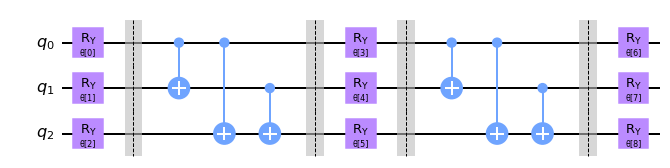
\includegraphics[width=\linewidth]{Artefact/Appendices/ansatz3-2.png}
    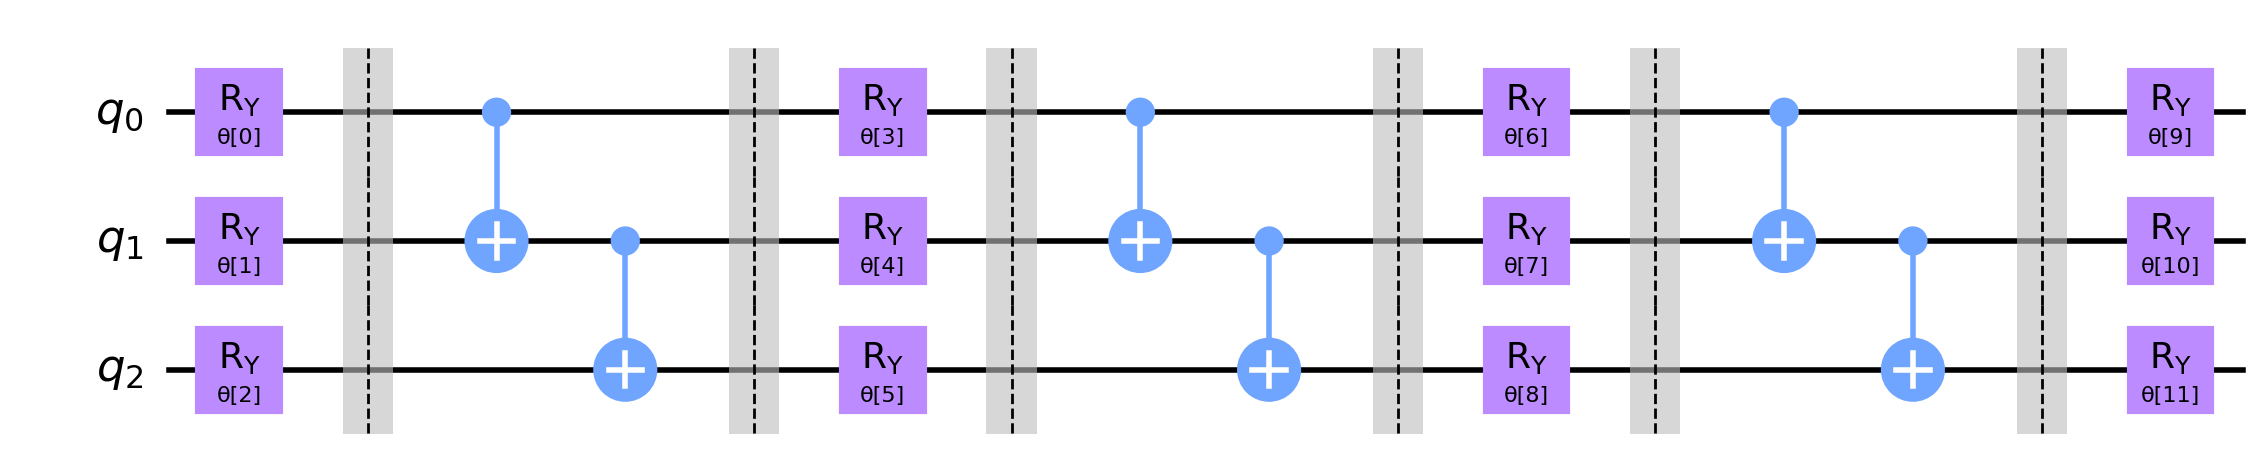
\includegraphics[width=\linewidth]{Artefact/Appendices/ansatz3-3.png}
    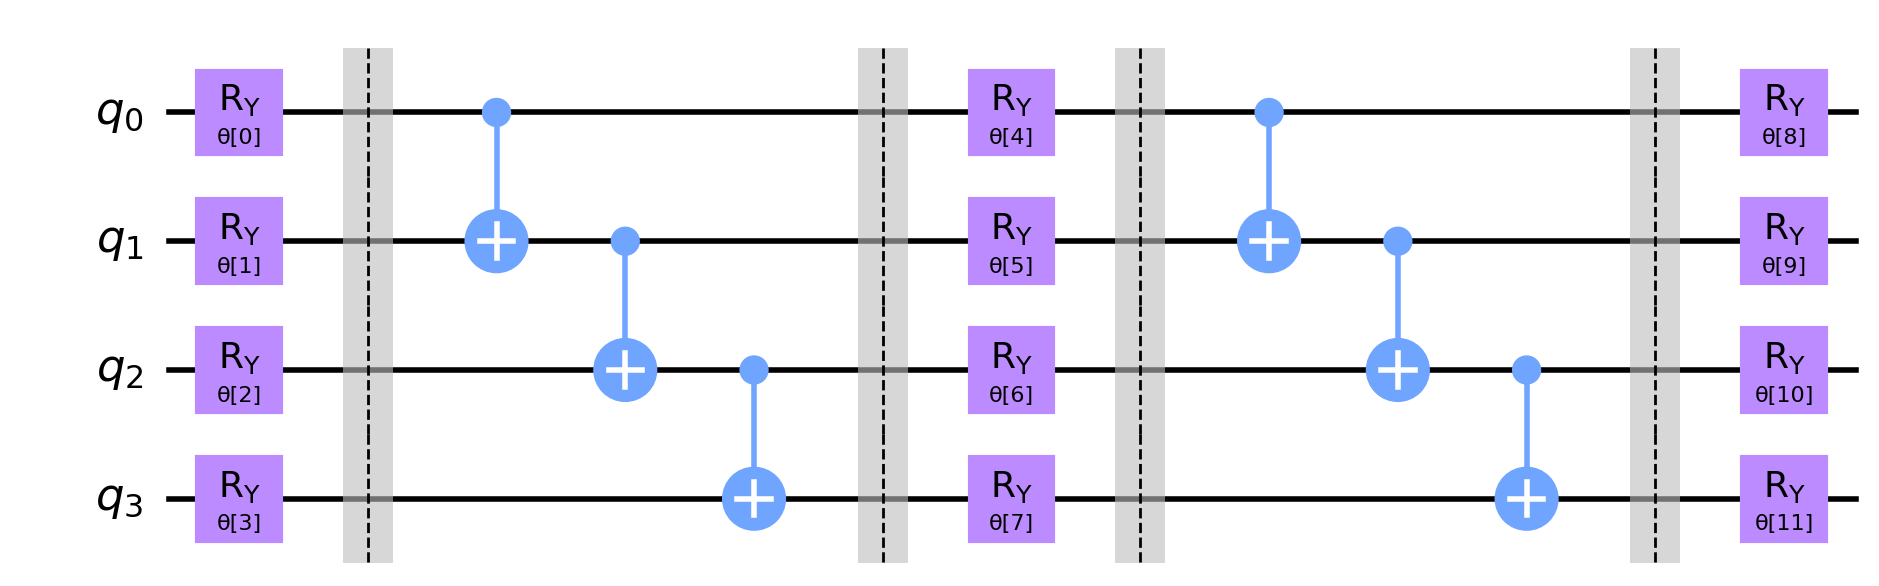
\includegraphics[width=\linewidth]{Artefact/Appendices/ansatz4-2.png}
    \caption{
        Samples of parameterised circuits generated by the Qiskit framework.
        The ansatz is a sequence of rotation layers and entanglement layers.
        All three: Real Amplitudes ansatz generated by Qiskit.
        Above: an ansatz of three qubits and two repetition layers.
        Middle: an ansatz of three qubits and three repetition layers.
        Below: an ansatz of four qubits and two repetition layers.
    }
    \label{Fig: Ansatz samples}
\end{figure}

For the case of identity block method, we will be using a customised ansatz, since reversing an ansatz would cancel the effect of the entanglement layer.
The customised ansatz are specialised to create identity blocks without losing the entanglement layers, section \ref{Sec: Method3} gives further discussion of this ansatz.